\section{Implicit Representation of Set Families}
\label{sec:fd-set-family}

\Cref{sec:cpig} introduced the concept of \emph{conditional predicate implications},
and presented an algorithm for inferring additional implications and counterexamples.
Let $\Omega$, called the \emph{ground set}, be the domain of predicates.
$\Omega$ is often, as in fair division, uncountably infinite.
This raises the question: how do we represent sets that implications and counterexamples
are conditioned on, for the purpose of computation?
\Cref{sec:cpig} briefly mentioned how to handle this:
define a finite set family $\Fcal \subseteq 2^{\Omega}$ that is represented implicitly,
and have all implications and counterexamples be conditioned on sets from $\Fcal$.
Moreover, given any $S, T \in \Fcal$, we need an efficient algorithm to
check if $S \subseteq T$.
But what do we mean by implicit representation?
And how do we implicitly represent $\Omega$ for the fair division problem?
In this section, we give precise answers to these questions.

\subsection{Representing Set Families as Mappings from Partial Orders}

\begin{definition}
\label{defn:set-family-repr}
A set family $\Fcal \subseteq 2^{\Omega}$ is \emph{represented by} a partial order $(P, \preceq)$
if there exists an order-preserving surjective mapping $f: P \to \Fcal$,
i.e., for all $S \in \Fcal$, there exists $x \in P$ such that $f(x) = S$,
and for all $x, y \in P$, we have $x \preceq y \implies f(x) \subseteq f(y)$.
\end{definition}

Note that the converse is not required to be true, i.e.,
$f(x) \subseteq f(y)$ need not imply $x \preceq y$.
Hence, if $P$ is an antichain, then $P$ trivially represents $\Fcal$.
However, such a representation is useless.
The more a representation captures the subset relations in $\Fcal$,
the better that representation is.

\begin{example}
Let $E$ be the set of even integers, i.e., $E \defeq \{2i: i \in \mathbb{Z}\}$,
and let $O$ be the set of odd integers, i.e., $O \defeq \{2i+1: i \in \mathbb{Z}\}$.
Then the set family $\Fcal \defeq \{E, O, \mathbb{Z}\}$ can be represented by
the partial order $(\{e, o, a\}, \{e \preceq e, a \preceq a, o \preceq o, e \preceq a, o \preceq a\})$,
where the corresponding mapping $f$ is given by $f(e) = E$, $f(o) = O$, and $f(a) = \mathbb{Z}$.
\end{example}

Hence, for the conditional predicate implication problem,
if we can represent a set family $\Fcal \subseteq 2^{\Omega}$
by a finite partial order $(P, \preceq)$,
then we can indirectly specify the sets that implications and counterexamples
are conditioned on by elements in $P$.
In fact, for computation, we do not even need to know the set $\Fcal$ and the mapping $f$;
we can just work with elements in $P$ instead.
In the algorithm for inferring additional implications and counterexamples,
we perform several checks of the form $S \subseteq T$, where $S, T \in \Fcal$.
We replace them with checks of the form $x \preceq y$, where $f(x) = S$ and $f(y) = T$.

\subsection{Partial Order for Fair Division Settings}

\Cref{sec:cpig} mentioned that to apply the conditional predicate implication framework
to the fair division problem, we let $\Omega$ be the set of all pairs $(\Ical, A)$,
where $\Ical$ is a fair division instance and $A$ is an allocation for $\Ical$.
We want our family $\Fcal \subseteq 2^{\Omega}$ to represent fair division settings.
Hence, we represent each set in $\Fcal$ by a 5-tuple, as specified in \cref{sec:settings}.
We now explain how to define a partial order on these 5-tuples,
and how to map each 5-tuple to a subset of $\Omega$.

\begin{definition}[Product order]
Let $((P_i, \preceq_i))_{i=1}^k$ be a sequence of partial orders.
Their \emph{product} is another partial order $(P, \preceq)$, where
$P \defeq \prod_{i=1}^k P_i \defeq \{(p_i)_{i=1}^k: p_j \in P_j \forall j \in [k]\}$
and $(p_1, \ldots, p_k) \preceq (q_1, \ldots, q_k)$ iff $p_i \preceq_i q_i$ for all $i \in [k]$.
\end{definition}

\begin{example}
The product of $(\mathbb{N}, \le)$ with itself is $(\mathbb{N}^2, \preceq)$,
where $(a_1, a_2) \preceq (b_1, b_2)$ iff $a_1 \le a_2$ and $b_1 \le b_2$.
\end{example}

\begin{figure*}[!htb]
\centering
\begin{subfigure}{0.4\textwidth}
    \centering
    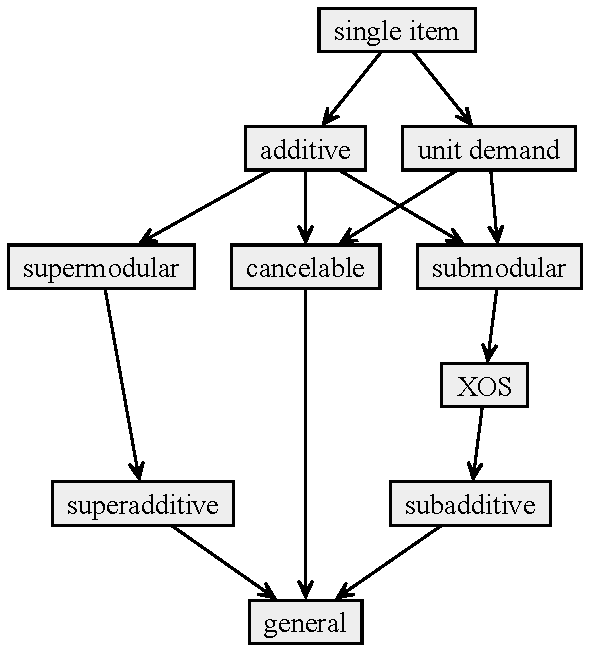
\includegraphics[width=\linewidth]{figs/valuation.pdf}
    \caption{Valuation function type}
\end{subfigure}
\hfill
\begin{subfigure}{0.59\textwidth}
    \centering
    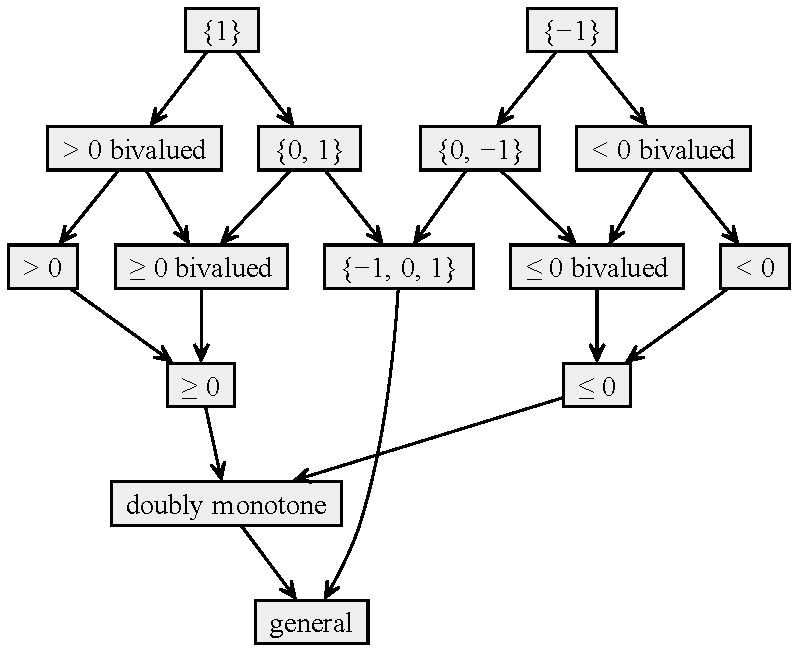
\includegraphics[width=\linewidth]{figs/marginal.pdf}
    \caption{Marginal values}
\end{subfigure}
\caption[Hasse diagrams of valuation function type and marginal values]{%
Partial orders for valuation function type and marginal values represented as \emph{Hasse diagrams},
i.e., for a DAG $G = (V, E)$, the corresponding partial order is $(V, \preceq)$,
where $u \preceq v$ iff there is a path from $u$ to $v$ in $G$.}
\label{fig:dag-posets}
\end{figure*}

Recall the 5 features of fair division from \cref{sec:settings}:
whether entitlements are equal,
whether there are only two agents,
whether agents have identical valuations,
valuation function type,
and marginal values.
%
We define a partial order for each of these 5 features.
The first three features are represented by the \emph{boolean} partial order:
$(\{\mathrm{true}, \mathrm{unknown}\}, \{\mathrm{true} \preceq \mathrm{unknown}, \mathrm{true} \preceq \mathrm{true}, \mathrm{unknown} \preceq \mathrm{unknown}\})$.
The partial orders for the last two features are given by \cref{fig:dag-posets}.
Let $(P, \preceq)$ be the product of these 5 partial orders.
%
For a fair division setting $s \in P$, let
$f(s) \defeq \{(\Ical, A): \Ical$ is an instance consistent with $s$,
$A$ is an allocation for $\Ical\}$, and $\Fcal \defeq \{f(s): s \in P\}$.
It is easy to check that $f$ is order-preserving and surjective.
This completes our description of how to map fair division settings to subsets of $\Omega$.

Note that $f$ is not injective. The settings
$s_1 \defeq (\mathrm{unknown}, \mathrm{unknown}, \mathrm{true}, \mathrm{additive}, \{1\})$
and $s_2 \defeq (\mathrm{unknown}, \mathrm{unknown}, \mathrm{unknown}, \mathrm{general}, \{1\})$
map to the same set in $\Fcal$, because if
each item's marginal value is 1, then valuations are identical and additive.
Querying the inference engine with $s_2$
may fail to infer implications that rely on additivity or identical valuations.
Note that $s_1 \preceq s_2$.
Among equivalent settings, querying the inference engine with a minimal setting
gives the most informative results, provided that counterexamples fed to the engine
are also conditioned on minimal settings.
